\newacronym{mri}{MRI}{magnet resonance imaging}
\newacronym{vocal}{VOCAL}{Virtual Organ Computer-aided Analysis}

In this section the clinical background of the data and the processing steps is verbalized. The source of the data and the different forms of data acquisition are especially important in order to understand why different processing steps have to be performed. Linking the visualization and the processing of the medical data to their origin and thinking about possible applications is also important for understanding the overall concept.

\section{Related data and data acquisition}

According to Huang and Zeng \cite{Huang2017} real-time \gls{3d} ultrasound imaging is a very well accepted technique in medicine, because it provides interactive feedback for the clinicians. Violea et. al. state that there are different issues when working with ultrasound data like noise or other visual artefacts \cite{Viola2013}. It is very important to have a precise navigation and visual feedback in order to acquire meaningful data with a high level of details \cite{Viola2013}. One problem in 3D ultrasound is that the perceivable volume might not be large enough to record the whole range of interest. This problem occurs in many cases for example when examining inner organs like the liver but it is also a very prominent issue when working with fetal data \cite{Viola2013, Lee1995ThreeMode}.\newline

The data delivered by 3D ultrasound can be seen as a cloud of data points aligned at a \gls{3d} grid. In case of a fetal examination they can represent various things like mother fluid, artefacts from the tissues which the signal of the ultrasound has to travel through or also organic tissue which is floating in the mother fluid as well as of course the fetus. The data points have to be characterized and it has to be clear which of them really belong to the fetus, obviously the object of interest. Having a look at the anatomy of the woman the data acquisition may be somehow tricky. The belly is very well exposed and it leads to beautiful pictures from one side but having a look at the other side of the fetus may be impossible. The ultrasound waves do not travel very well through hard tissue like bones and therefore the examination of the fetus through the back of a woman is not helpful. A schematic explanation how a fetal ultrasound investigation is carried out is depicted in Figure \ref{Fetal_Ultrasound}.\newline\newline

\begin{figure} [htb!]
    \centering
	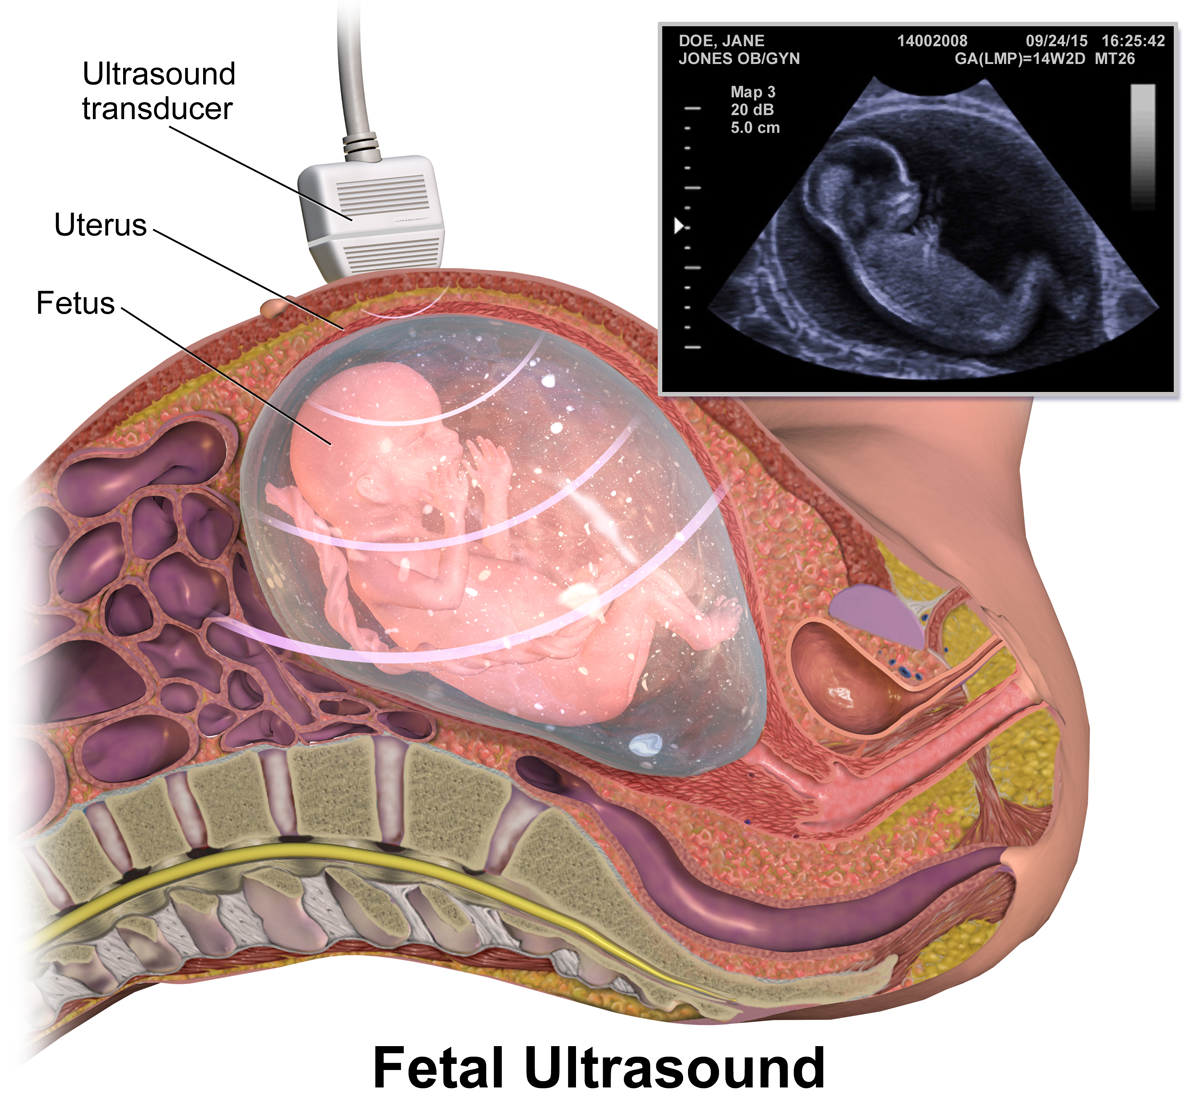
\includegraphics[width=12cm]{content/images/Fetal_Ultrasound}
	\caption{Schematic description of how a fetal ultrasound investigation is carried out including anatomical details of the pregnant woman \cite{BruceBlausFetalUltrasound}.}
	\label{Fetal_Ultrasound}
\end{figure}

\section{Analysis of the data}
\gls{2d}, \gls{3d} and also \gls{4d} ultrasound investigations are techniques which are without a doubt very important for the analysis of a fetus. Gathering insight of the fetal surface as well as the organs and the cardiovascular system are essential for supporting a healthy development.

\subsection{Organ analysis}

The development of the inner organs is a very important aspect in the early development of a human being. Many problems during the growth phase of the essential organs like the heart or the lungs are induce from the outside. Therefore in case of growth issues expectant mothers could be advised on how to avoid bad influences.

\subsubsection{Lung growth}

Moeglin et. al. state that various ultrasound techniques may be used to identify fetal lung growth \cite{Moeglin2005}. They write about using \gls{2d} and \gls{3d} ultrasound based approaches as well as \gls{mri} based techniques. The \gls{mri} based measurements are able to encounter more detailed analysis because they able to overcome the limitations of ultrasound based imaging but the downside is that the costs are higher, the patient compliance is lower and it is highly affected by the fetal movement \cite{Moeglin2005,Bonet-Carne2015QuantitativeMorbidity}.\newline\newline
Fetal lung volume might be measured using the \gls{vocal} software by General Electric Medical Systems KretzTechnik which is able to produce a \gls{3d} model of the lung. A representation of the graphical output of the software can be seen in Figure \ref{fig:fetal_lung_volumetry} \cite{Moeglin2005}.\newline

\begin{figure} [htb!]
    \centering
	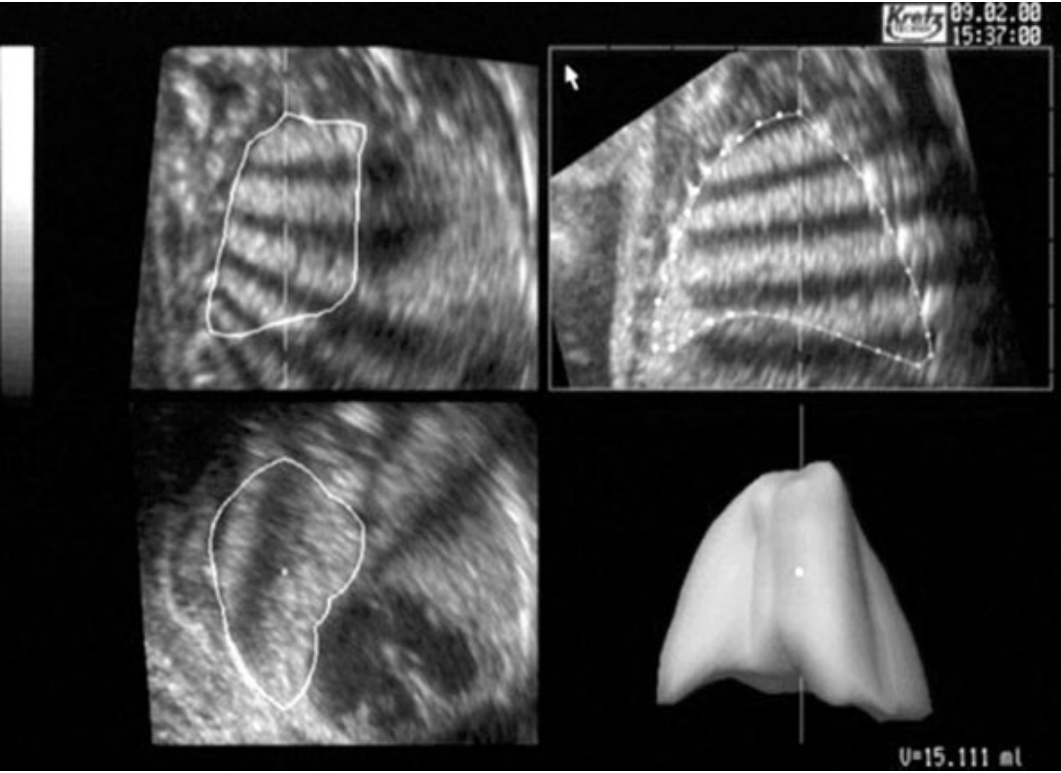
\includegraphics[width=12cm]{content/images/fetal_lung_volumetry}
	\caption{Output of the \gls{vocal} software using an rotation technique to estimate the fetal lung volumetry. The lung volume is estimated by rotating it around the vertical axis. In the lower right corner a produced 3D model of the lung can be seen \cite{Moeglin2005}.}
	\label{fig:fetal_lung_volumetry}
\end{figure}
\newpage
\subsubsection{Cardiovascular system}

The fetal cardiovascular system is also subject of analysis \cite{Yagel2007,Baschat2011ExaminationSystem,Dong2013PreliminaryAnomalies}. It suffers from congenital pathology most often \cite{Dong2013PreliminaryAnomalies}. \gls{3d} ultrasound and modern visualization techniques can for example be used in order to examine and visualize the inter ventricular septum \cite{Yagel2007}. Figure \ref{fig:septum} represents the ultrasound image and the surface rendering of the septum.

\begin{figure} [htb!]
    \centering
	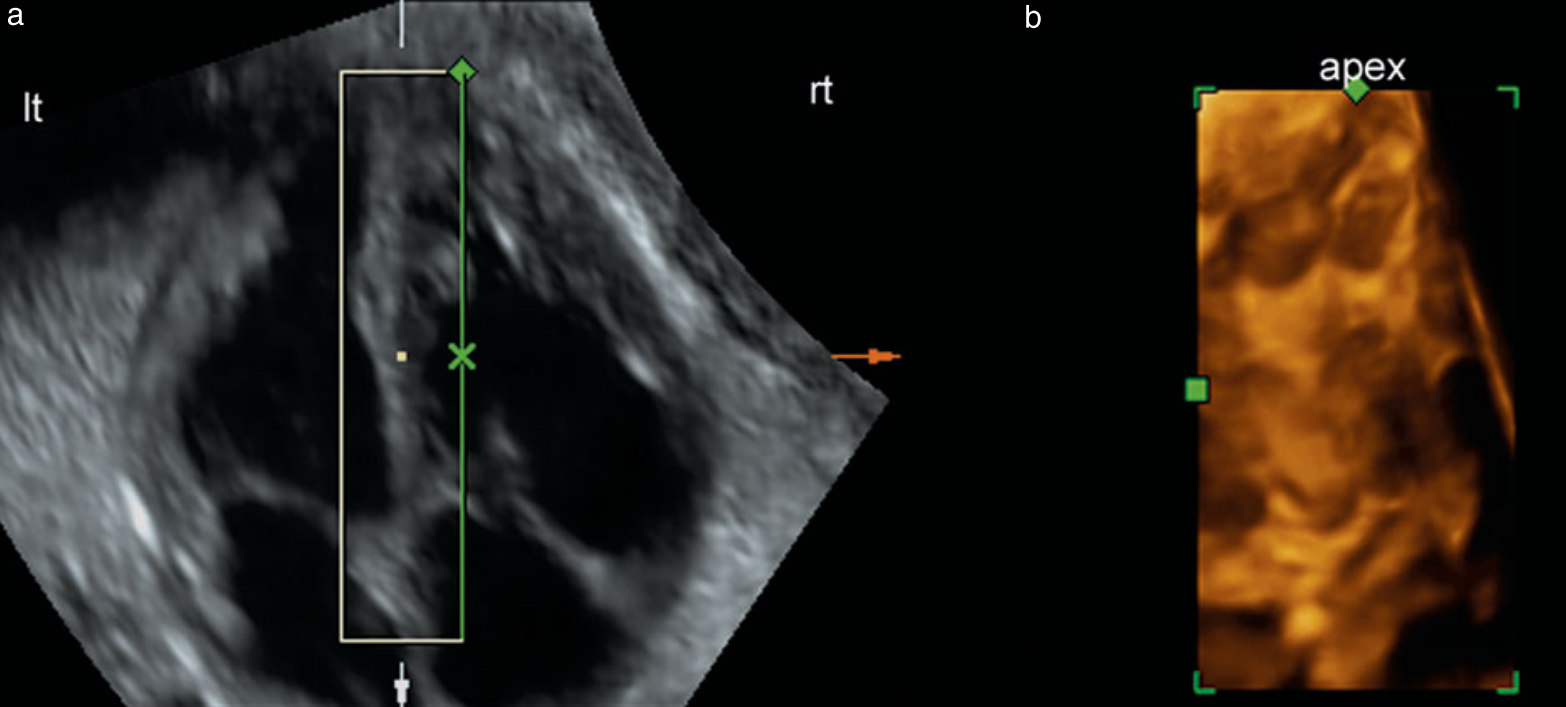
\includegraphics[width=13cm]{content/images/septum}
	\caption{Left left side of the image shows the ultrasound image of the heart and the interventricular septum is inside of the green box. The surface of the septum is visualized on the right side which might help doctors to examine for abnormalities \cite{Yagel2007}.}
	\label{fig:septum}
\end{figure}

Another important measurement at the cardiovascular level is to measure the cardiac output volume using Doppler evaluation \cite{Baschat2011ExaminationSystem}. Baschat shows in his paper that this technique may be used to examine the flow through different vessels in a fetus in order to find out if there is any occlusion or abnormality \cite{Baschat2011ExaminationSystem}. The author states that it is an essential tool for perinatal specialists for the generation of clinical diagnoses. Figure \ref{fig:cardioPulmonary} shows an example of how the output of such a Doppler evaluation may look like.

\begin{figure} [htb!]
    \centering
	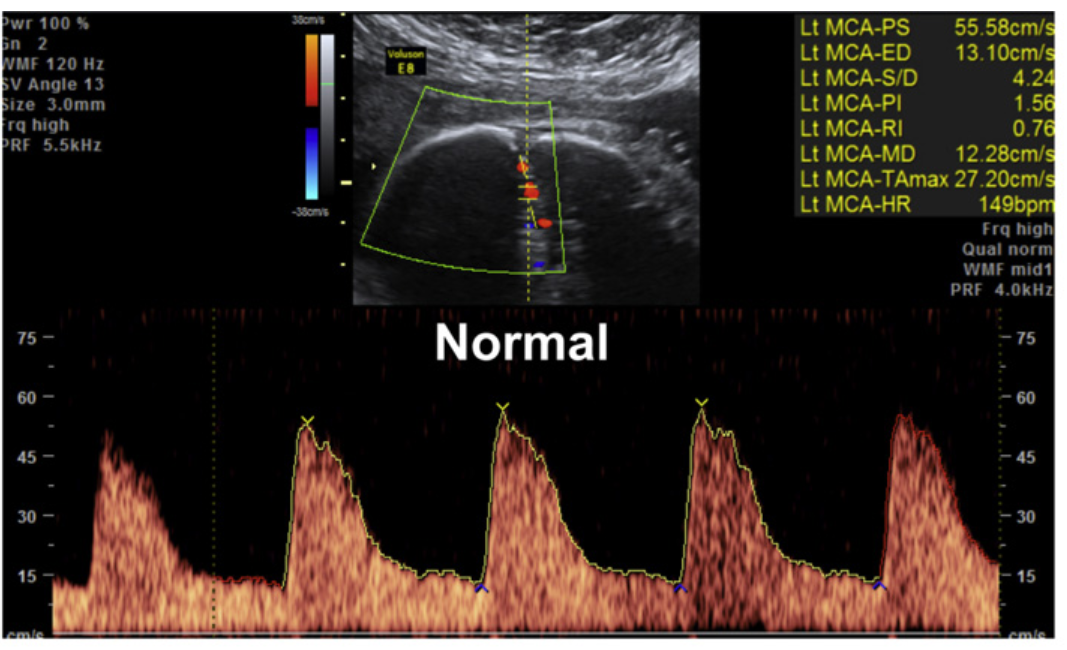
\includegraphics[width=13cm]{content/images/cardioPulmonary}
	\caption{Doppler signal of the middle cerebral artery of a fetus \cite{Baschat2011ExaminationSystem}.}
https://www.overleaf.com/project/5c7edf5a9c804c4085911acb	\label{fig:cardioPulmonary}
\end{figure}

\newpage
\subsection{Facial development}

Another very important aspect which can be examined using \gls{3d} ultrasound is the development of the face of the fetus. The information about facial deformations is not only important for obstetricians or paediatricians the surface visualization of the given data is also important when telling the parents \cite{Lee1995ThreeMode}. It can be somehow tough to explain them with words that their child is going to have deformations in the face but showing them makes it a lot easier to perceive. An example for such a facial surface visualization is depicted in Figure \ref{fig:face}.

\begin{figure} [htb!]
    \centering
	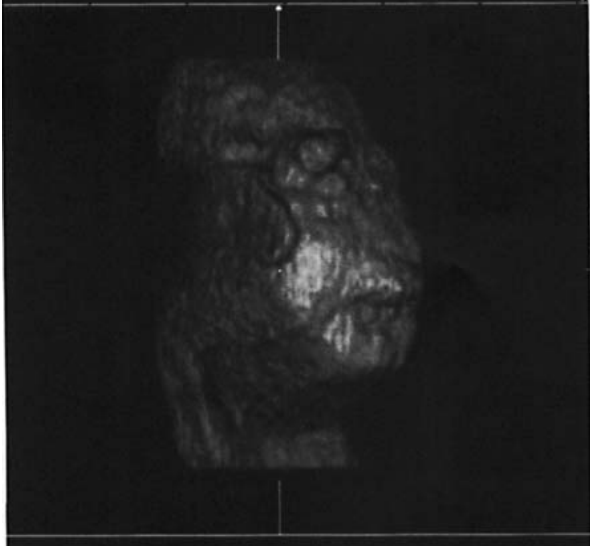
\includegraphics[width=10cm]{content/images/face}
	\caption{Ultrasound surface visualization of a male fetus in the \nth{30} week of pregnancy. The face does not show any regular facial structure \cite{Lee1995ThreeMode}.}
	\label{fig:face}
\end{figure}

\subsection{Fetal growth analysis}\label{subsct:fetalGrowth}

Fetal size measurement more general growth analysis is a well known topic and many different scientists have written about it \cite{Hadlock1984EstimatingParameters.,Schild2000FetalUltrasound,Loughna2009,Whitworth2014}.The size and the weight of the fetus is of a special interest for the clinicians in the birth preparation. Knowing what to expect can be very important during the birth. In earlier times the growth analysis has only taken the \gls{2d} images into account and the measurements where for example the following: \gls{crl} or \gls{hc}. Those are very well defined and Loughna et. al. perfectly illustrate how to measure them which may be seen in Figure \ref{fig:crlmeasurement} and Figure \ref{fig:hc} \cite{Loughna2009}. The head circumference is measured using the outer to outer biparietal diameter and the occipital-frontal diameter \cite{Loughna2009}.

\begin{figure}[htb!]
    \begin{minipage}{7cm}
        \centering
        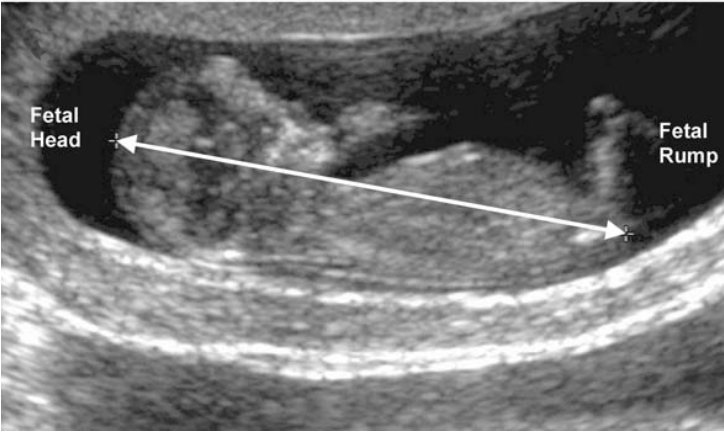
\includegraphics[width=7cm]{content/images/crlmeasurement}
        \caption{Crown-rump measurement of a fetus \cite{Loughna2009}.}
        \label{fig:crlmeasurement}
    \end{minipage}
    \hspace{0.02\textwidth}
    \begin{minipage}{7cm}
        \centering
        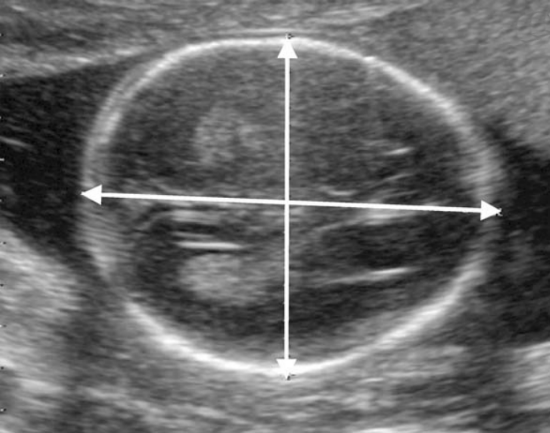
\includegraphics[width=5.35cm]{content/images/hc}
         \caption{Head circumference measurement  \cite{Loughna2009}.}
         \label{fig:hc}
    \end{minipage}
\end{figure}

\newpage
Another important measurement is the femur length. Hadlock et.al. state that the head circumference in combination with the femur length are a strong predictor of the fetal age \cite{Hadlock1984EstimatingParameters.} Knowledge about the age is essential in the fetal growth analysis because only with this information the growth is comparable to standardized tables like stated in \cite{Loughna2009}.\newline\newline

\gls{3d} ultrasound also plays a role in fetal growth analysis. Schild et.al. found out that using the three dimensional data produced by the \gls{3d} ultrasound, weight estimation can be enhanced \cite{Schild2000FetalUltrasound}. They also use the influence of soft tissue in order to find out more about the constitution of the fetus and the effects of this on the weight \cite{Schild2000FetalUltrasound}. \newline

The growth analysis is done over the whole pregnancy of the woman starting with the \nth{13} week and ending with the \nth{42} \cite{Loughna2009}. In this period of time the growth is calculated using the formulas presented in the paper of Loughna et.al. and than compared with standardized tables \cite{Loughna2009}. The problem which may arise here is that those measurements take some time and have to be performed for every investigation. A standardized position or pose of the fetus may be helpful to not only visualize the growth of the fetus in the different stages of the pregnancy but also analytically calculate it.  

